\section{E3: Nutzen der Adaption}
\label{app:report_e3}
\subsection*{Setup}
\begin{itemize}
\item \textbf{Lauf:} e3\_\allowbreak{}007
\item \textbf{Stichtage:} SF6: 02.12.2016, SF7: 13.01.2017, SF8: 20.02.2017
\item \textbf{Szenarien:} ramp\_\allowbreak{}28\_\allowbreak{}strong, ramp\_\allowbreak{}28\_\allowbreak{}down\_\allowbreak{}strong, scaled\_\allowbreak{}strong, scaled\_\allowbreak{}down\_\allowbreak{}strong, jeweils ab dem Stichtag, dazu der Kontrolllauf
\item \textbf{Systeme:} SYS1, SYS3
\item \textbf{Sprachmodell:} ministral-3:8b, Prompt v30, ohne Kalender (CTX0)
\item \textbf{Fenster:} 40 Tage vor und 60 Tage ab dem Stichtag
\item \textbf{Commit:} f647560 (mit lokalen Änderungen)
\end{itemize}

\subsection*{Kriterien der Teilfrage 3 aus E3}
\begin{tablang}{W{1.18} W{0.65} W{1.71} W{0.45}}{Kriterium & Ziel & Ergebnis & erfüllt}
Tagesfehler SYS3 minus SYS1 & < 0, belastbar & \textminus{}0,9 W, 2 Standardfehler 6,9 W, nicht belastbar & nein \\
Meldungen SYS3 minus SYS1 & < 0 je 30 Tage & \textminus{}7,9 & ja \\
\end{tablang}

\subsection*{Kennzahlen ab dem Zurücksetzen, SYS3 gegen SYS1}
\begin{tablang}{W{1.76} W{0.59} W{0.65}}{Kennzahl & SYS1 & SYS3}
Fälle mit Zurücksetzen & 0 von 12 & 11 von 12 \\
Tagesfehler [W] & 90,9 & 90,0 \\
Differenz [W] & - & \textminus{}0,9 \\
2 Standardfehler [W] & - & 6,9 \\
gepaarte Tage & - & 347 \\
Differenz belastbar & - & nein \\
Meldungstage & 113 & 24 \\
Meldungen je 30 Tage & 10,1 & 2,1 \\
Differenz Meldungen & - & \textminus{}7,9 \\
Zurücksetzen im Kontrolllauf & 0 & 0 \\
\end{tablang}

\subsection*{Tagesfehler und Meldungstage je Woche ab dem Zurücksetzen, alle Fälle}
\begin{tablang}{V{0.57} V{0.57} V{1.14} V{1.14} V{1.00} V{1.29} V{1.29}}{Woche & Fälle & Tagesfehler SYS3 [W] & Tagesfehler SYS1 [W] & Differenz [W] & Meldungstage SYS1 & Meldungstage SYS3}
1 & 11 & 101,6 & 85,0 & 16,5 & 45 & 6 \\
2 & 9 & 89,7 & 91,7 & \textminus{}2,0 & 34 & 1 \\
3 & 9 & 98,4 & 116,4 & \textminus{}18,0 & 14 & 1 \\
4 & 9 & 78,5 & 89,1 & \textminus{}10,6 & 5 & 8 \\
5 & 6 & 75,2 & 66,9 & 8,3 & 7 & 5 \\
6 & 5 & 109,2 & 105,1 & 4,1 & 8 & 3 \\
7 & 5 & 48,6 & 54,5 & \textminus{}5,9 & 0 & 0 \\
8 & 1 & 67,1 & 62,9 & 4,2 & 0 & 0 \\
\end{tablang}

\subsection*{Hinweise}
\begin{itemize}
\item Tag = Entscheidungstag seit dem Stichtag, an Tag n wird Tag n\textminus{}1 eingeordnet
\item Fall = Stichtag \texttimes{} Szenario. Ein Fall geht in die Auswertung ein, wenn SYS3 die Historie zurücksetzt. Erkennung und Einordnung prüfen E1 und E2
\item Tagesfehler: ab dem Tag des Zurücksetzens, denn die Prognose desselben Tages enthält es schon. SYS1 wird auf denselben Tagen gepaart und setzt nie zurück
\item Meldungen: Tage nach dem Zurücksetzen, bei beiden Systemvarianten auf denselben Tagen. Als Meldung zählen peak, new\_\allowbreak{}pattern, measurement\_\allowbreak{}error
\item Woche ab dem Zurücksetzen: Fälle mit spätem Zurücksetzen haben weniger Tage im Fenster und fallen in späteren Wochen heraus, die Spalte Fälle zeigt das
\item Kontrolllauf über das ganze Fenster, jede Meldung dort ist unbegründet, jedes Zurücksetzen unnötig
\item Das Kriterium zur Abwesenheit (Tagesfehler nach der Rückkehr) stammt aus den Läufen von E2
\item Mehrlaufzeit: Laufzeit von SYS3 minus SYS1 je Szenario, geteilt durch die Aufrufe des Sprachmodells. Grobe Schätzung, die Zeit eines Aufrufs wird nicht einzeln gemessen
\item belastbar: Betrag der Differenz größer als 2 Standardfehler der gepaarten Differenzen, grobe Faustregel
\end{itemize}
\begin{center}
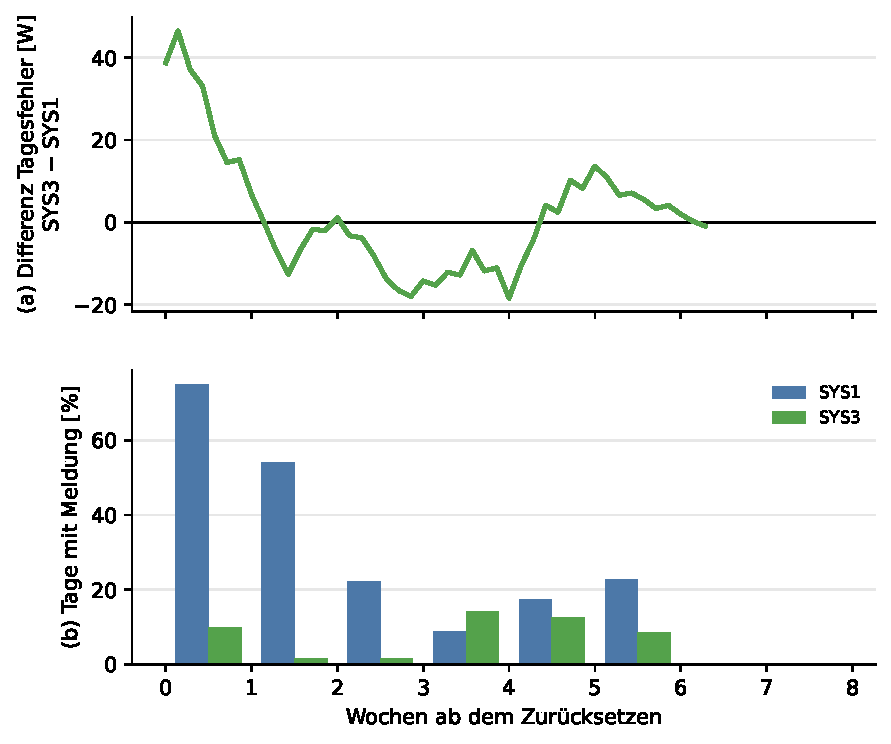
\includegraphics[width=\linewidth]{e3_weeks.pdf}
\end{center}

\subsection*{Weitere Tabellen}

\begin{landscape}
\subsubsection*{Tagesfehler und Meldungstage je Woche ab dem Zurücksetzen, je Szenario}
\begin{tablang}[\footnotesize\setlength{\tabcolsep}{3pt}]{W{1.41} V{0.54} V{0.54} V{1.08} V{1.08} V{0.94} V{1.21} V{1.21}}{Szenario & Woche & Fälle & Tagesfehler SYS3 [W] & Tagesfehler SYS1 [W] & Differenz [W] & Meldungstage SYS1 & Meldungstage SYS3}
ramp\_\allowbreak{}28\_\allowbreak{}strong & 1 & 3 & 134,8 & 86,5 & 48,3 & 11 & 0 \\
ramp\_\allowbreak{}28\_\allowbreak{}strong & 2 & 3 & 144,1 & 148,6 & \textminus{}4,5 & 11 & 1 \\
ramp\_\allowbreak{}28\_\allowbreak{}strong & 3 & 3 & 157,3 & 188,8 & \textminus{}31,5 & 5 & 1 \\
ramp\_\allowbreak{}28\_\allowbreak{}strong & 4 & 3 & 106,2 & 107,7 & \textminus{}1,5 & 5 & 1 \\
ramp\_\allowbreak{}28\_\allowbreak{}strong & 5 & 2 & 97,6 & 86,8 & 10,8 & 7 & 2 \\
ramp\_\allowbreak{}28\_\allowbreak{}strong & 6 & 2 & 122,8 & 119,6 & 3,2 & 8 & 2 \\
ramp\_\allowbreak{}28\_\allowbreak{}strong & 7 & 2 & 59,8 & 58,6 & 1,2 & 0 & 0 \\
ramp\_\allowbreak{}28\_\allowbreak{}down\_\allowbreak{}strong & 1 & 3 & 72,4 & 94,1 & \textminus{}21,7 & 14 & 2 \\
ramp\_\allowbreak{}28\_\allowbreak{}down\_\allowbreak{}strong & 2 & 2 & 53,2 & 52,6 & 0,6 & 2 & 0 \\
ramp\_\allowbreak{}28\_\allowbreak{}down\_\allowbreak{}strong & 3 & 2 & 50,4 & 51,0 & \textminus{}0,6 & 0 & 0 \\
ramp\_\allowbreak{}28\_\allowbreak{}down\_\allowbreak{}strong & 4 & 2 & 41,3 & 37,3 & 4,0 & 0 & 1 \\
ramp\_\allowbreak{}28\_\allowbreak{}down\_\allowbreak{}strong & 5 & 1 & 69,0 & 70,3 & \textminus{}1,4 & 0 & 0 \\
scaled\_\allowbreak{}strong & 1 & 2 & 160,4 & 115,2 & 45,1 & 6 & 0 \\
scaled\_\allowbreak{}strong & 2 & 1 & 57,1 & 62,0 & \textminus{}5,0 & 7 & 0 \\
scaled\_\allowbreak{}strong & 3 & 1 & 133,5 & 180,3 & \textminus{}46,8 & 3 & 0 \\
scaled\_\allowbreak{}strong & 4 & 1 & 127,7 & 207,1 & \textminus{}79,5 & 0 & 6 \\
scaled\_\allowbreak{}strong & 5 & 1 & 80,7 & 67,9 & 12,8 & 0 & 0 \\
scaled\_\allowbreak{}strong & 6 & 1 & 144,7 & 131,2 & 13,4 & 0 & 0 \\
scaled\_\allowbreak{}strong & 7 & 1 & 23,7 & 54,2 & \textminus{}30,6 & 0 & 0 \\
scaled\_\allowbreak{}down\_\allowbreak{}strong & 1 & 3 & 66,8 & 61,0 & 5,8 & 14 & 4 \\
scaled\_\allowbreak{}down\_\allowbreak{}strong & 2 & 3 & 70,4 & 70,8 & \textminus{}0,3 & 14 & 0 \\
scaled\_\allowbreak{}down\_\allowbreak{}strong & 3 & 3 & 59,7 & 66,2 & \textminus{}6,4 & 6 & 0 \\
scaled\_\allowbreak{}down\_\allowbreak{}strong & 4 & 3 & 53,0 & 55,1 & \textminus{}2,1 & 0 & 0 \\
scaled\_\allowbreak{}down\_\allowbreak{}strong & 5 & 2 & 52,3 & 45,2 & 7,1 & 0 & 3 \\
scaled\_\allowbreak{}down\_\allowbreak{}strong & 6 & 2 & 77,9 & 77,5 & 0,4 & 0 & 1 \\
scaled\_\allowbreak{}down\_\allowbreak{}strong & 7 & 2 & 57,2 & 52,2 & 5,0 & 0 & 0 \\
scaled\_\allowbreak{}down\_\allowbreak{}strong & 8 & 1 & 67,1 & 62,9 & 4,2 & 0 & 0 \\
\end{tablang}
\end{landscape}

\subsubsection*{Fälle je Stichtag und Szenario}
\begin{tablang}{W{0.79} W{1.37} V{1.18} V{0.79} V{1.05} W{0.92} V{0.92}}{Stichtag & Szenario & Zurücksetzen an Tag & gepaarte Tage & Differenz Tagesfehler [W] & belastbar & Differenz Meldungen je 30 Tage}
SF6 & ramp\_\allowbreak{}28\_\allowbreak{}strong & 17 & 44 & \textminus{}6,0 & nein & \textminus{}12,6 \\
SF6 & ramp\_\allowbreak{}28\_\allowbreak{}down\_\allowbreak{}strong & 28 & 33 & \textminus{}3,8 & nein & \textminus{}6,6 \\
SF6 & scaled\_\allowbreak{}strong & 58 & 3 & 115,2 & ja & 0,0 \\
SF6 & scaled\_\allowbreak{}down\_\allowbreak{}strong & 18 & 43 & \textminus{}0,2 & nein & \textminus{}5,7 \\
SF7 & ramp\_\allowbreak{}28\_\allowbreak{}strong & 16 & 45 & 1,9 & nein & \textminus{}9,5 \\
SF7 & ramp\_\allowbreak{}28\_\allowbreak{}down\_\allowbreak{}strong & 38 & 23 & \textminus{}3,8 & nein & \textminus{}4,1 \\
SF7 & scaled\_\allowbreak{}strong & 14 & 47 & \textminus{}16,6 & nein & \textminus{}6,5 \\
SF7 & scaled\_\allowbreak{}down\_\allowbreak{}strong & 33 & 28 & \textminus{}2,9 & nein & \textminus{}4,4 \\
SF8 & ramp\_\allowbreak{}28\_\allowbreak{}strong & 35 & 26 & 23,5 & nein & \textminus{}9,6 \\
SF8 & ramp\_\allowbreak{}28\_\allowbreak{}down\_\allowbreak{}strong & 56 & 5 & \textminus{}34,3 & nein & \textminus{}22,5 \\
SF8 & scaled\_\allowbreak{}strong & - & - & - & - & - \\
SF8 & scaled\_\allowbreak{}down\_\allowbreak{}strong & 11 & 50 & 3,5 & ja & \textminus{}8,6 \\
\end{tablang}

\subsubsection*{Kontrolllauf: Meldungen und Zurücksetzen ohne Anlass}
\begin{tablang}{W{0.92} W{0.77} V{0.54} V{1.38} V{1.38}}{Stichtag & System & Tage & Meldungstage & Zurücksetzen}
SF6 & SYS1 & 101 & 9 & 0 \\
SF6 & SYS3 & 101 & 9 & 0 \\
SF7 & SYS1 & 101 & 8 & 0 \\
SF7 & SYS3 & 101 & 8 & 0 \\
SF8 & SYS1 & 101 & 5 & 0 \\
SF8 & SYS3 & 101 & 5 & 0 \\
\end{tablang}

\subsubsection*{Laufzeit des Sprachmodells}
\begin{tablang}{W{0.82} W{1.43} V{0.75} V{1.09} V{1.23} V{0.68}}{Stichtag & Szenario & Aufrufe & Ausfalltage & Mehrlaufzeit [s] & je Aufruf [s]}
SF6 & Kontrolllauf & 36 & 0 & 690,2 & 19,2 \\
SF6 & ramp\_\allowbreak{}28\_\allowbreak{}strong & 41 & 0 & 734,4 & 17,9 \\
SF6 & ramp\_\allowbreak{}28\_\allowbreak{}down\_\allowbreak{}strong & 32 & 0 & 588,0 & 18,4 \\
SF6 & scaled\_\allowbreak{}strong & 55 & 0 & 1007,1 & 18,3 \\
SF6 & scaled\_\allowbreak{}down\_\allowbreak{}strong & 46 & 0 & 831,6 & 18,1 \\
SF7 & Kontrolllauf & 61 & 0 & 1137,2 & 18,6 \\
SF7 & ramp\_\allowbreak{}28\_\allowbreak{}strong & 40 & 0 & 737,4 & 18,4 \\
SF7 & ramp\_\allowbreak{}28\_\allowbreak{}down\_\allowbreak{}strong & 35 & 0 & 652,4 & 18,6 \\
SF7 & scaled\_\allowbreak{}strong & 49 & 0 & 914,1 & 18,7 \\
SF7 & scaled\_\allowbreak{}down\_\allowbreak{}strong & 37 & 0 & 697,9 & 18,9 \\
SF8 & Kontrolllauf & 55 & 0 & 1019,1 & 18,5 \\
SF8 & ramp\_\allowbreak{}28\_\allowbreak{}strong & 53 & 0 & 974,1 & 18,4 \\
SF8 & ramp\_\allowbreak{}28\_\allowbreak{}down\_\allowbreak{}strong & 75 & 0 & 1375,3 & 18,3 \\
SF8 & scaled\_\allowbreak{}strong & 79 & 0 & 1439,8 & 18,2 \\
SF8 & scaled\_\allowbreak{}down\_\allowbreak{}strong & 59 & 0 & 1076,2 & 18,2 \\
alle & alle & 753 & 0 & 13874,8 & 18,4 \\
\end{tablang}
